\chapter{FET projects and social media}
This chapter presents an overview of the presence of FET projects on social media. Ut enim ad minim veniam, quis nostrum exercitationem ullam corporis suscipit laboriosam, nisi ut aliquid ex ea commodi consequatur. Quis aute iure reprehenderit in voluptate velit esse cillum dolore eu fugiat nulla pariatur. Excepteur sint obcaecat cupiditat non proident, sunt in culpa qui officia deserunt mollit anim id est laborum.

\section{Data set}
This thesis focuses on the communication activity of the FET projects funded within Horizon 2020. The list of such projects was downloaded on 15th July 2017 from CORDIS, the main portal of the European Commission on results of EU-funded research projects. It consists of 151 projects and is reported in Appendix \ref{List_of_FET_projects}. The Appendix reports information on the budget, start and end date of the project as well as the considered online communication channels. FET projects approved after 15th July 2017 are not considered in this thesis.  

Not all projects in the list were considered for this thesis. Excluded classes of projects were the Flagships and Launchpad as they are not representative of the FET projects in terms of communication effort. Flagship projects were disregarded due to their budget. As it is far superior compared to the other FET projects, the Human Brain Project and the Graphene projects are two outliers and cannot be considered representative of the typical FET project. Launchpad projects were disregarded as they have very limited budget to invest on communication and because communicating the results is not their priority. In fact, as mentioned in section ... , they mainly focus on finding applications to the market of results achieved by previous FET projects. Finally, projects which started after 1st February 2017 were disregarded as the time period between such date and the date when the list was downloaded was considered not sufficient to fully develop and launch the project's communication strategy. The exclusion of such projects shrinked the data set from 151 projects to ... . The list of excluded projects is available in Appendix \ref{Specific_lists_of_FET_projects}.

For some analyses in this thesis, the data set of ... project was divided into three sub-groups. The three subgroups were then compared among each other to highlight the differences in the communications strategies among different classes of projects. One subgroup includes the ...number... FET projects in the field of quantum technologies. The second group consists of the ...number... projects active in the development of high performance computing and the transition to the exascale. The third group comprises the ...number... remaining projects. The list of projects in the quantum technologies and HPC groups are reported in appendix \ref{Specific_lists_of_FET_projects}.     

\section{Considered channels} 
There exist disparate channels suitable for communication purposes. Those offering the widest audience are provided by the web. Examples are websites and social media. For this reason, FET projects consider the internet as one of the main pillars of their communication strategy.

Different approaches can be considered to assess the use of online communication channels made by FET projects. One quantitative estimate is provided by the fraction of projects active on specific platforms. For this thesis, the following communication channels were considered:   

\begin{description}
 \item [Website] The website is the online channel offering the highest degree of freedom to the owner. It allows the owner to personalise the content, the overall structure and the graphic impact.
 \item [Facebook] Facebook is the most used social media. It offers direct interaction among users and activities are recorded. Nevertheless, it is mainly designed for free time.  
 \item [Twitter] Twitter is very effective for short science-related communication. However, it requires high posting rates and offers less personal interaction compared to Facebook.
 \item [Linkedin] Linkedin is ideal for professional content and enables the creation of closed groups. Nevertheless, interaction among users and outreach within the groups are limited.
 \item [YouTube] YouTube is the world's main platform for video sharing. It provides a very direct communication channel with effective monitoring tools. On the other hand, it does not offer straightforward engagement channels and finding appropriate content may be difficult for users.
 \item [Instagram]Instagram has a very active and rapidly growing community. It requires pictures with strong visual content and offers a limited interaction among users.
 \item [ResearchGate] ResearchGate offers the possibility to share documentation and engage in scientific discussions with researchers. As members are mainly scientists, the community which can be reached is significantly smaller compared to other social networks.  
\end{description}

For each FET projects in appendix \ref{List_of_FET_projects}, a search was performed to find out which online communication platforms among the aformentioned ones had been considered. This search included contacting each project directly. Not for all project was possible to find a contact and in some cases it was not possible to receive an answer (dare numero). For this projects, the author performed a desk search. It cannot be excluded that the desk search did not find all accounts activated by the projects on the aformentioned social channels. It is therefore highly probable that the list of accounts is not complete. Hence, the results presented in this thesis can be considered as inferior limits.   

\begin{figure}[!t] 
 \begin{center}
 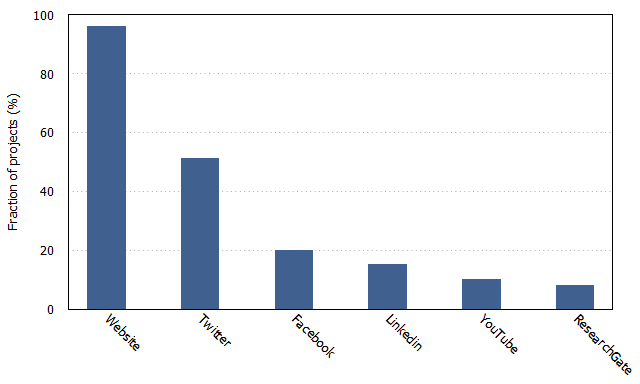
\includegraphics[scale=0.4]{Images/Social_media.png}
 \caption{Duration and allocated budget of Europe's Research and Innovation programmes (also known as Framework Programmes, FP). Budgets are expressed in billion Euros.}
 \label{FP_funds}
 \end{center}
\end{figure}